%!TEX root = ../dissertation.tex
\chapter{Introduction}
\label{ch:intro}

In the last years the scientific community made significant progress
in the development of models for solving computer vision and natural
language processing tasks. The reasons behind those outstanding
advancements are manifold. In first place, the constant increase of
computational resources allows to exploit complex models which can
capture intricate behavior. Secondly, the availability of new data
speed-up the learning process in terms of how we can benefit from
available information. However, the joint understanding of both
modalities is still an hard task, specially if we constraint the
problem within a deliberately simple and human-like environment.

Both visual and language modalities are required for solving
interesting, challenging and community worthwhile problems such us
visual question answering \cite{kafle2017visual}, image retrieval
\cite{gordo2016deep, radenovic2016cnn}, robotic navigation
\cite{thomason2017guiding} and visual grounding
\cite{plummer2015flickr30k,datta2019align2ground,wang2019phrase,wang2020maf,rigoni2021better}.
Among these, visual grounding task is a fundamental building block and
can be used to postulate other tasks as a variation of the latter. A
first abstract definition for visual grounding could be:

\begin{quote}
    \textit{The task of locating the content of the image referenced
    by a given sentence.}
\end{quote}

Take for example the image in Fig.~\ref{fig:dog-playing-with-ball}
(top) and the phrase ``A collie plays with a white ball in a field of
green grass''. We can think to many solutions for the visual grounding
problem given that input. A first approach would be to grossly
localize the subject of the phrase in the image, thus, practically
speaking, to draw a coarse box around the dog playing with the ball
(red box). Another solution instead would be to localize the ball, the
dog and the ground distinctly (yellow, red and blue boxes),
identifying precise regions of the image and draw precise boxes among
interested objects. Both two solutions are legal and belong to the
visual grounding field. The former is known as referring expression
grounding (REG) while the latter as phrase grounding (PG). The main
difference between the two is the grain used to solve the problem, and
this has significant impacts on how we can approach the problem and
the relevance for other tasks.

\begin{figure}
  \centering
  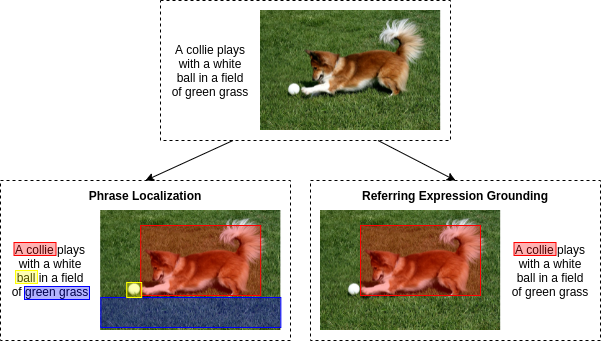
\includegraphics[width=0.8\textwidth]{figures/dog-playing-with-ball.png}
  \caption[Phrase localization versus referring expression grounding
  problem]{Phrase localization versus referring expression grounding
  problem.}
  \label{fig:dog-playing-with-ball}
\end{figure}

With the availability of large datasets
\cite{plummer2015flickr30k,kazemzadeh2014referitgame}, many different
solution for the visual grounding task has been proposed in
literature, but most of them relies on expensive annotations. We argue
that this technique cannot scale and is becoming a critical bottleneck:
it is hard and expensive to collect grounding information while very
simple to collect images with their descriptions. Also, the way humans
learn phrase localization is by assembling prior knowledge instead of
memorize a mapping between textual and image examples.

This encourages us to investigate the visual grounding task under the
weakly supervised setting. In weakly supervised scenario, the
available ground truth is a shallow information which links a
description with its own image and vice-versa. On the contrary, the
fully supervised setting provide also the information between noun
phrases and objects in image, while in unsupervised settings no ground
truth is available.

In this work we propose a simple model that learns from concept
similarity. The goal is to solve phrase localization problem under
weakly supervised settings. Given a noun phrase, we define it's
concept as the most important word in the phrase, while, given a
bounding box we define it's class as the label, among a dictionary of
labels, predicted by an object detector for that bounding box. The
concept similarity is the similarity between the phrase concept and
bounding box class. Here, the key idea is that the head of the phrase
should be very similar (semantically speaking) to the content of the
bounding box and thus, to its class. 

Our model is straightforward. First of all, we gather image features
from the object detector and we compute five additional features
representing bounding box top left and bottom right corners and area
(spatial features). We then project those features to a subspace,
performing a dimensionality reduction. Regarding the text, we first
represent words in phrase by pretrained embeddings and then we encode
the phrase through a recurrent neural network with LSTM cells. Our
predictions are the results of the cosine similarity between projected
image features and the last LSTM hidden neuron. On those prediction we
apply concept similarity, which empower related proposals to be most
likely the grounded boxes. Finally, the model is optimized for
maximizing similarity on sentences that do describe and image, while
minimizing similarity of sentences that do not describe and image.

In this work we show how extra information from object detector, such
us the probability distribution on proposal classes, can be
effectively employed in a grounding model although our basic model
components and simple loss. Results confirm that the strategy is
effective, performing comparably on both Flickr30k Entities and
ReferIt datasets.

This dissertation is structured as follows:
\begin{itemize}
    \item Ch.~\ref{ch:background} introduces all background notions
    required to understand our work;
    \item Ch.~\ref{ch:related-works} overviews the literature mainly
    in phrase grounding, focusing on weakly supervised works;
    \item Ch.~\ref{ch:model} reports our model implementation;
    \item Ch.~\ref{ch:experiments} shows our results in comparison
    with State-of-the-Art approaches; 
    \item Ch.~\ref{ch:conclusion} sums up our considerations and
    outline some possible improvements to our approach.
\end{itemize}
